\documentclass{beamer}

\usepackage{amssymb,amsmath}
\usepackage{graphicx}
\usepackage{url}
\usepackage{color}
\usepackage{pagenote}[continuous,page]
\usepackage{relsize}		% For \smaller
\usepackage{url}			% For \url
\usepackage{epstopdf}	% Included EPS files automatically converted to PDF to include with pdflatex

%For MindMaps
% \usepackage{tikz}%
% \usetikzlibrary{mindmap,trees,arrows}%

%%% Color Definitions %%%%%%%%%%%%%%%%%%%%%%%%%%%%%%%%%%%%%%%%%%%%%%%%%%%%%%%%%
%\definecolor{bordercol}{RGB}{40,40,40}
%\definecolor{headercol1}{RGB}{186,215,230}
%\definecolor{headercol2}{RGB}{80,80,80}
%\definecolor{headerfontcol}{RGB}{0,0,0}
%\definecolor{boxcolor}{RGB}{186,215,230}

%%% Save space in lists. Use this after the opening of the list %%%%%%%%%%%%%%%%
%\newcommand{\compresslist}{
%	\setlength{\itemsep}{1pt}
%	\setlength{\parskip}{0pt}
%	\setlength{\parsep}{0pt}
%}

%\setbeameroption{show notes on top}

% You should run 'pdflatex' TWICE, because of TOC issues.

% Rename this file.  A common temptation for first-time slide makers
% is to name it something like ``my_talk.tex'' or
% ``john_doe_talk.tex'' or even ``discrete_math_seminar_talk.tex''.
% You really won't like any of these titles the second time you give a
% talk.  Try naming your tex file something more descriptive, like
% ``riemann_hypothesis_short_proof_talk.tex''.  Even better (in case
% you recycle 99% of a talk, but still want to change a little, and
% retain copies of each), how about
% ``riemann_hypothesis_short_proof_MIT-Colloquium.2000-01-01.tex''?

\mode<presentation>
{
  \usetheme{CambridgeUS}		% bem bacana - menu superior
  \usecolortheme{default}		% branco, azul clarinho
  \useoutertheme{default}
  \useinnertheme{circles}
  \setbeamercovered{invisible}
}

\beamertemplatenavigationsymbolsempty

%% Better looking blocks
\setbeamercolor{block title alerted}{use=structure,fg=black,bg=red!80!black}
\setbeamercolor{block body alerted}{use=structure,fg=black,bg=white!90!black}

\setbeamercolor{block title}{use=structure,fg=black,bg=blue!60!white}
\setbeamercolor{block body}{use=structure,fg=black,bg=white!90!black}

\usepackage[english]{babel}
\usepackage[latin1]{inputenc}
\usepackage{subfigure}

\usepackage{times}
\usepackage[T1]{fontenc}

%% makes the ppagenote command for figure references at the end.
\makepagenote
\renewcommand{\notenumintext}[1]{}
\newcommand{\ppagenote}[1]{\pagenote[Page \insertframenumber]{#1}}


\usepackage{tikz}
\usetikzlibrary{arrows,shapes}

\title[GB13604]{GB13604 - Maths for Computer Science}
\subtitle[]{Lecture 6 -- Counting Part I}
\author[Claus Aranha]{Claus Aranha\\{\footnotesize caranha@cs.tsukuba.ac.jp}}
\institute[COINS]{College of Information Science}
\date[2018-11-14]{2018-11-14\\{\tiny Last updated \today}}

\tikzstyle{vertex}=[circle,fill=black!25,minimum size=10pt,inner sep=0pt]
\tikzstyle{blue vertex}=[circle,fill=blue!100,minimum size=10pt,inner sep=0pt]
\tikzstyle{red vertex}=[circle,fill=red!100,minimum size=10pt,inner sep=0pt]
\tikzstyle{yellow vertex}=[circle,fill=yellow!100,minimum size=10pt,inner sep=0pt]
\tikzstyle{edge} = [draw,thick,-]
\tikzstyle{pedge} = [draw,thick,.]
\tikzstyle{red edge} = [draw, thick,-,red!50]
\tikzstyle{black edge} = [draw, line width=2pt,-,black!20]
\tikzstyle{weight} = [font=\smaller]

\begin{document}

\begin{frame}
  \maketitle

  \begin{center}
    {\smaller This course is based on Mathematics for Computer Science, Spring
    2015, by Albert Meyer and Adam Chlipala, Massachusetts Institute
    of Technology OpenCourseWare.}
    
    
\includegraphics[width=0.2\textwidth]{../img/by-nc-sa}
  \end{center}
\end{frame}

\section{Introduction}

\begin{frame}
  \frametitle{Week 6 and 7 summary}

  {\larger
    {\bf Counting}

    \bigskip

    \begin{itemize}
    \item \structure{Sums and Products}
    \item \structure{Asymptotics}
    \item \alert{Counting with Bijections}
    \item \alert{Repetitions and Binomial Theorem}
    \item \alert{Pigeonhole Principle}
    \end{itemize}
  }
\end{frame}

\section{Sums and Products}

\begin{frame}
  \frametitle{Sums for Children}
  
  {\larger
    Next two lectures: Talking about \structure{sums} and \structure{counting}.
    
    \bigskip
    
    \begin{block}{Middle School Classwork:}
      \begin{equation*}
        89 + 102 + 115 + 128 + \ldots + 440 + 453 + 466
      \end{equation*}
    \end{block}

    \bigskip      
    It is said that \alert{Gauss} found a quick solution for this
    problem at \alert{9 years old}:
    \begin{itemize}
    \item \structure{30 numbers, each 13 greater than the previous one.}
    \end{itemize}
  }
\end{frame}

\begin{frame}
  \frametitle{Sums for Children}

  {\larger
    
    \begin{itemize}
    \item $89 + (89+13) + \ldots + (89+28\times13) +(89+29\times13)$
    \item $F + (F+d) + \ldots + (L-d) + L = A$
    \item<2-> $L + (L-d) + \ldots + (F+d) + F = A$
    \item<3-> \structure{$(F+L) + (F+L) + \ldots + (F+L) + (F+L) = 2A$}
    \end{itemize}

    \bigskip

    \begin{onlyenv}<3->
      \begin{equation}
        A = \frac{(F+L)}{2} \times (\text{\# of terms})
      \end{equation}
    \end{onlyenv}

    \begin{onlyenv}<4->
      \begin{equation}
        A = \frac{(1+n)}{2} \times (n)
      \end{equation}
    \end{onlyenv}
    
  }
\end{frame}
  

\begin{frame}
  \frametitle{Why Counting?}

  {\larger

    \begin{itemize}
    \item \structure{Counting} techniques help understand the structure of numbers:
    \item We will study three different sums:
      \begin{itemize}
      \item Arithmetic Sums
      \item Geometric Sums
      \item Harmonic Sums
      \end{itemize}  
    \end{itemize}

    \bigskip

    \begin{block}{Motivation for this unit}
      Counting techniques can be used to estimate \structure{upper
        bounds} and \structure{lower bounds} of computer complexity in
      algorithms.
    \end{block}
  }
\end{frame}

\subsection{Geometric Sums}

\begin{frame}
  \frametitle{Arithmetic Sums and Geometric Sums}

  {\larger

    \begin{itemize}
    \item \structure{Arithmetic Sums}: Add a fixed value to each element\\
      $A = (a+0d) + (a+d) + (a+2d) + \ldots + (a+nd)$

      \bigskip

    \item \structure{Geometric Sums}: Multiply a fixed value to each element\\
      $G = (kx^0) + (kx^1) + (kx^2) + \ldots + (kx^n)$
    \end{itemize}
    
  }
  
\end{frame}

\begin{frame}
  \frametitle{Closed Form for the Geometric Sum}

  {\larger
    \begin{itemize}
    \item $A = 1 + 2 + 3 + \ldots + n = \frac{n(n+1)}{2}$, $G = 1 + x + x^2 + \ldots + x^n = ?$

      \bigskip

    \item<2-> $G = 1 + x + x^2 + \ldots + x^n$
    \item<2-> $xG = x + x^2 + x^3 + \ldots + x^{n+1}$

      \bigskip

    \item<3-> $G = 1 + x + x^2 + \ldots + x^n$ 
    \item<3-> $-xG = - x - x^2 - \ldots - x^{n+1}$
      
    \item<3-> $G-xG = 1 $\hspace{2cm}$-x^{n+1}$
    \item<3-> $G(1-x) = 1 - x^{n+1}$, $G = \frac{1-x^{n+1}}{1-x}$      
    \end{itemize}
  }
\end{frame}

\begin{frame}
  \frametitle{Closed Form for the Geometric Sum}

  {\larger
    \begin{itemize}
    \item The {\bf Proof By Induction} can show if a formula is
      correct, but does not show \alert{where the formula comes from}

      \bigskip

    \item The {\bf Perturbation Method} can be used to find
      \structure{closed forms} for sums.
    \end{itemize}
  }
\end{frame}


\begin{frame}
  \frametitle{Infinite Geometric Sums}

  {\larger

    \begin{itemize}
    \item \structure{Geometric Sum}:

      \begin{equation}
        G_n = \frac{1-x^{n+1}}{1-x}
      \end{equation}
      
    \item \structure{Geometric {\bf Series}}:
      \begin{equation}
        \lim_{n\rightarrow\inf}G_n = \frac{1-\lim_{n\rightarrow\inf}x^{n+1}}{1-x} = \frac{1}{1-x}
      \end{equation}
      \hfill(Provided that $|x| < 1$)
    \end{itemize}
    
  }
\end{frame}

\begin{frame}
  \frametitle{Application: Calculating Loans}

  {\larger

    {\bf Problem:} I pay you \structure{100\$ in 1 year} if you
    \alert{pay me X\$ now}

    \bigskip

    How do we calculate a fair amount for \alert{X}?
    \begin{itemize}
    \item <2-> My bank will pay me 3\% \structure{interest}\\
      \hfill{\emph{bankrate} b ::= 1.03}
    \item <3-> If I deposit \alert{X\$} now, I will have
      \alert{$b\times X$\$} in 1 year.
    \item <3-> So I will not lose money if $b\times X \geq 100$\\
      \hfill $X \geq 100/1.03 =$ \structure{97.09}
    \end{itemize}
    
  }  
\end{frame}

\begin{frame}
  \frametitle{The future worth of money}
  
  {\larger
    \begin{itemize}
    \item 1\$ next year is worth \$0.9709 now.
      \bigskip

    \item \structure{r\$} last year is worth 1 today, if $r ::= 1/b$
      \bigskip

    \item $n$ in two years is worth
    \item $nr$ in one year, and it is worth
    \item $nr^2$ today.
    \end{itemize}

    \vfill

    \begin{center}
      \structure{$n$} paid in $k$ years is \alert{worth $nr^k$ today},
      where \structure{$r ::= 1/\text{bankrate}$}
    \end{center}
  }
\end{frame}

\begin{frame}
  \frametitle{Annuity}

  {\larger
    {\bf Insurance Company}: I will pay you 100\$ for 10 years,
    if you pay me \$Y now. \structure{How much should Y be?}

    \bigskip

    \begin{itemize}
    \item The Insurance company needs:
    \item $100r + 100r^2 + 100r^3 + \ldots + 100r^{10}$
    \item<2-> Insurance = $100r(1+r+r^2+\ldots+r^9)$
    \item<2-> $I = 100r \times \frac{1-r^{10}}{1-r} = 853.02$
    \end{itemize}

  }
\end{frame}

\subsection{Book Stacking}

\begin{frame}
  \frametitle{Problem: Book Stacking}

  \begin{center}
    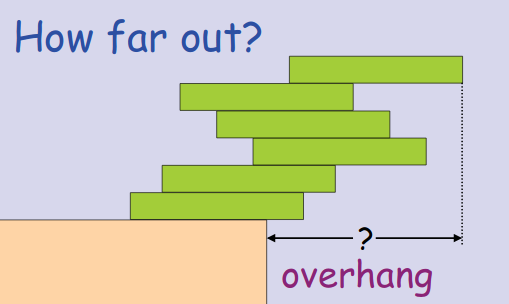
\includegraphics[width=0.8\textwidth]{../img/bookstack1}
  \end{center}
  
\end{frame}

\begin{frame}
  \frametitle{Book Stacking Problem}

  {\large

    \begin{itemize}
    \item All books have size 1.
    \item For 1 book: \structure{Center of Mass} is 0.5\\
      \hfill 1-book overhang is 0.5.
      \bigskip
    \item What about $n$ books?
      
    \end{itemize}

    \begin{center}
      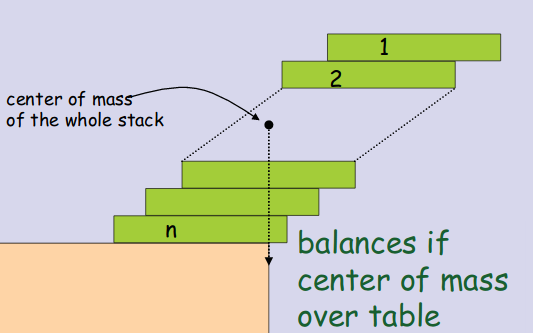
\includegraphics[width=0.6\textwidth]{../img/bookstack2}
    \end{center}
  }
\end{frame}

\begin{frame}
  \frametitle{Book Stacking Problem}
  \begin{center}
    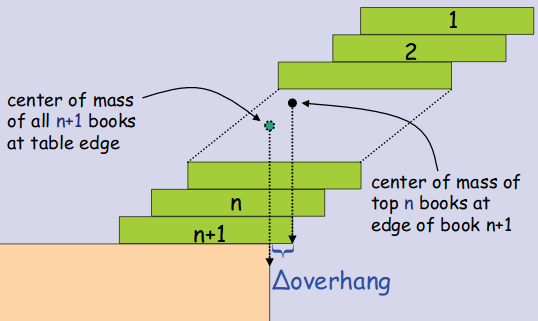
\includegraphics[width=0.6\textwidth]{../img/bookstack3}
  \end{center}

  {\larger $\Delta$-overhang ::= distance between CoM of $n$ books and
    CoM of the $n+1$ book.  }
\end{frame}

\begin{frame}
  \frametitle{$\Delta$-overhang}

  {\larger
    From physics, we know that:
    \begin{equation}
      \Delta = \frac{1}{2(n+1)}
    \end{equation}
    
    \begin{itemize}
    \item $B_n ::=$ overhang of $n$ books
    \item $B_1 = 1/2$
    \item $B_{n+1} = B_n + \frac{1}{2(n+1)}$
      \bigskip
      
    \item $B_n = 1/2(1+1/2+1/3+\ldots+1/n)$\\
      \hfill(This is harmonic Sum!)
    \end{itemize}
  }
\end{frame}

\begin{frame}
  \frametitle{How big can the overhang get?}

  {\larger
    
    It turns out that by increasing the number of $n$ books, we
    can make $1/2H_n$ as big as necessary.

    \vfill

    So there is no upper limit for the size of the overhang, if you
    position the books \alert{very carefully} and know integrals.
  }
\end{frame}

%% TODO: Include slides about Integral Theorem (for upper and lower limits)
%% TODO: Include slides about calculating bounds for Factorials

\section{Asymptotics}

\begin{frame}
  \begin{center}
    {\huge
      Asymptotics
    }
  \end{center}
\end{frame}

\begin{frame}
  \frametitle{Study of Asymptotics}

  {\larger
    \begin{itemize}
    \item How fast do expressions grow?
      \bigskip
      
    \item What is the maximum/minimum size of an expression?
      \bigskip
      
    \item How can we compare two expressions as they get more complex?
    \end{itemize}

    \bigskip

    We will look at \structure{four notations} that describe the
    relationship between the {\bf growth of functions}.

  }
\end{frame}

\begin{frame}
  \frametitle{Asymptotic Equivalence}

  {\larger

    Def: \structure{$f(n) \sim g(n)$}: \hfill(f(n) is asymptotically equal to g(n))

    \bigskip

    \begin{equation}
      \lim_{n\to\infty}\frac{f(n)}{g(n)} = 1
    \end{equation}

    {\bf Example:}
    \begin{itemize}
    \item $n^2 \sim n^2+n$ because...
    \item $\lim_{n\to\infty}\frac{n^2+n}{n} = \lim_{n\to\infty} \frac{1}{n} + 1 = 1$
    \end{itemize}
    
  }
\end{frame}

\begin{frame}
  \frametitle{Asymptotic Equivalence}

  {\larger

    {\bf Lemma:} $\sim$ is symmetric \hfill($f \sim g \implies g\sim f$)

    \begin{itemize}
    \item Let $f \sim g$ be true, is $g \sim f$ true too?
    \item $\lim \frac{g}{f} = \lim \frac{1}{(f/g)}$
    \item $\lim \frac{1}{(f/g)} = \frac{1}{\lim(f/g)} = \frac{1}{1} = 1$
    \item $f \sim g \implies g\sim f$\hfill$\blacksquare$
    \end{itemize}

  }
\end{frame}

\begin{frame}
  \frametitle{Asymptotic Equivalence}

  {\larger

    {\bf Transitivity:} Suppose $f \sim g$ and $g \sim h$. Prove $f \sim h$

    \bigskip

    \begin{equation}
      1 = \lim\frac{f}{g} = \lim\frac{f/h}{g/h} = \frac{\lim(f/h)}{\lim(g/h) = 1} = \lim\frac{f}{h} 
    \end{equation}

    \vfill

    {\bf Colorary:} $\sim$ is an \structure{equivalence relation}

    \begin{itemize}
    \item \alert{important} $sim$ is a relation \alert{on functions}
    \item $f(n) \sim g(n)$ does not care about \structure{particular
      values} of f(n) or g(n). ($f \sim g$)
    \end{itemize}
    
  }
\end{frame}

\begin{frame}
  \frametitle{Little Oh: $o(\cdot)$ -- Asymptotically Smaller}

  {\larger
    {\bf Definition:} $f(n) = o(g(n))\iff \lim_{n\to\infty}\frac{f(n)}{g(n)} = 0$

    \bigskip

    {\bf Example:}
    \begin{itemize}
    \item $n^2 = o(n^3)$
    \item $\lim_{n\to\infty}\frac{n^2}{n^3} = \lim_{n\to\infty}\frac{1}{n} = 0$
    \end{itemize}

    \bigskip

    {\bf Lemma:} $o(\cdot)$ defines a \structure{strict partial order}    
  }
\end{frame}

\begin{frame}
  \frametitle{Big Oh: $O(\cdot)$ -- Asymptotic Order of Growth}

  {\larger
    {\bf Definition:} $f(n) = O(g(n))$
    \begin{equation}
      \limsup_{n\to\infty}\frac{f(n)}{g(n)} < \infty
    \end{equation}

    \vfill
    
    \begin{itemize}
    \item The limit of f(n)/g(n) is \structure{finite}.
    \item Could be 0, could be 1, could be something else.
    \item Why \structure{limsup} not \structure{lim}? Ignore this for now.

      \bigskip

    \item {\bf Example}: $3n^2 = O(n^2)$ because $\lim\frac{3n^2}{n^2} = \lim3 = 3$
    \end{itemize}
    
  }
\end{frame}

\begin{frame}
  \frametitle{Why do we like $O(\cdot)$ so much?}

  {\larger
    \begin{itemize}
    \item What O() means is that \structure{constant factors} don't matter.
    \item Only \structure{rate of growth} matters.

      \bigskip

    \item When we talk about {\bf execution time}, if the hardware changes,
      only a \structure{constant factor} changes.

      \bigskip
      
    \item Slow algorithms will still be slow (for bigger data!) even if
      the hardware changes.
    \end{itemize}
    
  }
\end{frame}

\begin{frame}
  \frametitle{Theta: $\Theta(\cdot)$ -- Same Order of Growth}

  {\larger

    {\bf Definition}:
    \begin{equation}
      f = \Theta(g) \iff f = O(g) \land g = O(f)
    \end{equation}

    \bigskip

    {\bf Lemma}: $\Theta$ is an equivalence relation.
  }
  
\end{frame}

\begin{frame}
  \frametitle{Asymptotics: Intuitive Summary}

  {\larger

    \begin{itemize}
    \item $f\sim g$ \hfill f and g nearly equal;
      \bigskip

    \item $f = o(g)$ \hfill f much less than g;
      \bigskip

    \item $f = O(g)$ \hfill f is about $\leq$ g;
      \bigskip

    \item $f = \Theta(g)$ \hfill f is about equal to g;
    \end{itemize}

    
  }
\end{frame}

\subsection{Asymptotic Properties}

\begin{frame}
  \frametitle{Asymptotic Properties}

  {\larger

    \begin{itemize}
    \item If $f \sim g$ or $f = o(g)$ then $f = O(g)$
      \bigskip
      
    \item If $f = o(g)$ then $g \neq O(f)$\\
      \hfill ($\lim f/g = 0 \implies \lim g/f = \infty$)
      \bigskip
    \end{itemize}
  }
\end{frame}

\begin{frame}
  \frametitle{Big Oh $O(\cdot)$ and limsup}

  {\larger
    {\bf Alternate Definition:} $f(n) = O(g(n))$

    \begin{equation}
      \exists c,n_0, \forall n \geq n_0, f(n) \leq c\cdot g(n)
    \end{equation}

    \begin{center}
      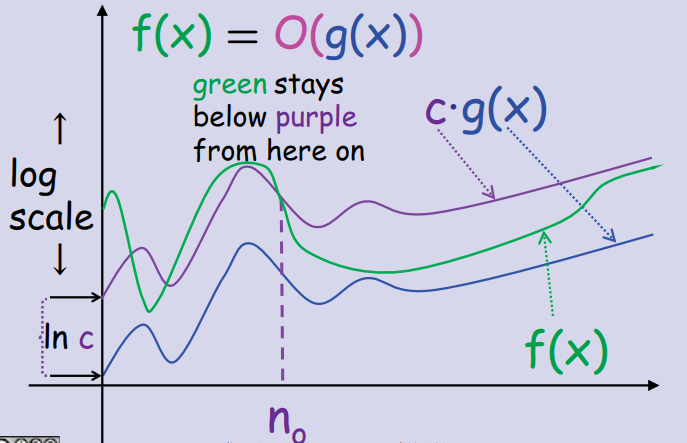
\includegraphics[width=0.6\textwidth]{../img/bigOh}
    \end{center}
    
  }
\end{frame}

\begin{frame}
  \frametitle{Big Oh $O(\cdot)$ and limsup}

  {\larger
    \begin{itemize}
    \item Why is \structure{limsup} necessary in the first definition?
    \item Suppose $f \leq 2g$ then $f = O(g)$ but $f/g$ has no limit.
      \bigskip

    \item {\bf Example:} $f(n) = (1+\sin^2(\frac{n\pi}{2}))\times g(n)$
      \bigskip
      
    \item The \structure{limit} of $f/g$ in this expression alternates
      between 1 and 2.
    \item On the other hand, the \structure{limsup} of $f/g$ is 2.
    \end{itemize}
  }
\end{frame}

\begin{frame}
  \frametitle{A few more facts about asymptotics}

  {\larger

    \begin{itemize}
    \item {\bf Lemma:} $x^a = o(x^b)$ if a < b\\
      \hfill because $\lim\frac{x^a}{x^b} = \lim\frac{1}{x^{a-b}}$ and $a-b > 0$
      \bigskip

    \item {\bf Lemma:} $\ln(x) = o(x^\epsilon)$ for $\epsilon > 0$\\
      \hfill (logarithms grow slower than roots)
    \end{itemize}

    {\bf Proof:}
    \begin{itemize}
    \item $1/y \leq y$ for $y \geq 1$, so $\int_1^z \frac{1}{y}dy \leq \int_1^z ydy$
    \item $\ln(z) \leq \frac{z^2}{2}$ for $z \geq 1$, so let $z =
      \sqrt{x^\delta}$, (for some $\delta > 0$)
    \item $\frac{\delta\ln(x)}{2} \leq \frac{x^\delta}{2}$, but
      $x^\delta = o(x^\epsilon)$ for $\delta < \epsilon$
    \item So $\delta\ln(x) = o(x^\epsilon)$\hfill $\blacksquare$
    \end{itemize}

  }
\end{frame}

\begin{frame}
  \frametitle{Asymptotic Blunders -- Be careful!}

  {\larger

    \begin{itemize}
    \item ``$\cdot = O(\cdot)$'' defines a \structure{binary relation}.\\
      \hfill \alert{Do not write O(x) = x!!}
      \begin{itemize}
      \item If $x = O(x)$ and $O(x) = x$...
      \item But $2x = O(x)$ and $O(x) = x$... so $2x = x$?????
      \end{itemize}

      \bigskip

    \item Big Oh is \structure{not a lower bound}.\\
      \hfill \alert{Do not write: ``f is at least $O(n^2)$''}
      \begin{itemize}
      \item If you want to say that $n^2$ is a \structure{lower bound} of f...
      \item $n^2 = O(f)$
      \end{itemize}
      
    \end{itemize}
  }  
\end{frame}

\begin{frame}
  \frametitle{Asymptotic Blunders -- Be careful!}

  {\larger
    \begin{itemize}
    \item {\bf False Proof:} $\sum^n_{i=1}i = O(n)$\\
      \hfill(We know that $\sum^n_{i=1}i = n(n+1)/2)$
      \bigskip

    \item Any constant is O(1): $0 = O(1), 1 = O(1), 2 = O(1) \ldots$
    \item So, $i = O(1)$
    \item So, $\sum^n_{i=1}i = O(1) + O(1) + O(1) + O(1) \ldots$
    \item So, $\sum^n_{i=1}i = nO(1) = O(n)$\hfill (???)
    \end{itemize}

    \vfill

    \alert{$O(\cdot)$ is not a quantity! Do not do arithmetic with it!}

  }
\end{frame}


\section{Conclusion}
\begin{frame}
  \frametitle{End of Class -- Class Summary}

  {\larger

    \begin{itemize}
    \item Sums: Arithmetic, Geometric, Harmonic, and Closed Forms

      \bigskip
    \item Asymptotic Notation: $\sim$, o(), O(), $\Theta$()       
    \end{itemize}

  }
\end{frame}

\end{document}
